% NOTA EDITORIAL: capítulo não incluído em main.tex nesta revisão. Conteúdo científico absorvido por chapters/04_datasets.tex (Capítulo 3, "Dados, desenho experimental e proveniência"). Arquivo mantido apenas como registro histórico.

\chapter{METODOLOGIA EXPERIMENTAL}

\section{Notação}

Considere um vetor padronizado de $d$ canais de informação,
\begin{equation}
  X=(X_1,\ldots,X_d),
\end{equation}
e um alvo binário $Y\in\{0,1\}$. Um conjunto de índices $I\subseteq\{1,\ldots,d\}$ determina o subconjunto de canais
\begin{equation}
  S_I=\{X_i:i\in I\}.
\end{equation}
A coleção de todos os subconjuntos não vazios é denotada por $\mathcal{S}$, com $|\mathcal{S}|=2^d-1$. O classificador é indicado por $f$, o braço experimental por $g$, o número de amostras de treinamento por classe por $n$ e a replicação Monte Carlo por $r$.

Para uma observação de teste $(x_t,y_t)$, a perda utilizada é o erro de classificação. Se o teste fixo possui $m$ observações, a perda da replicação é
\begin{equation}
  \widehat{L}^{(g)}_{S_I,f,r}(n)
  =\frac{1}{m}\sum_{t=1}^{m}
  \mathbf{1}\!\left\{\widehat{Y}^{(g,S_I,f)}_{t,r}(n)\neq y_t\right\}.
  \label{eq:replication-loss}
\end{equation}
Após $R_n$ replicações concluídas para aquele tamanho amostral, a estimativa principal é
\begin{equation}
  \overline{L}^{(g)}_{S_I,f}(n)
  =\frac{1}{R_n}\sum_{r=1}^{R_n}\widehat{L}^{(g)}_{S_I,f,r}(n).
  \label{eq:mean-loss}
\end{equation}
O simulador calcula perda empírica no teste; não estima erro de treinamento, erro de Bayes ou perda teórica.

\section{Padronização e espaço de modelagem}

Para cada canal $j$, a média $\widehat{\mu}_j$ e o desvio-padrão $\widehat{\sigma}_j$ são calculados somente nos dados reais de treinamento. As observações são transformadas por
\begin{equation}
  Z_j=\frac{X_j-\widehat{\mu}_j}{\widehat{\sigma}_j}.
  \label{eq:zscore}
\end{equation}
O mesmo par de parâmetros é aplicado ao teste real. Essa ordem é necessária para impedir que estatísticas do teste influenciem o treinamento dos classificadores, a parametrização dos geradores ou a calibração. A padronização também evita que canais com escalas numericamente maiores dominem classificadores sensíveis à escala, como SVM linear e Regressão Logística \cite{pedregosa2011}.

Uma mudança conceitual em relação aos experimentos idealizados anteriores é que os modelos geradores são parametrizados no espaço padronizado e produzem as amostras sintéticas nesse mesmo espaço. Assim, médias, covariâncias e componentes não representam diretamente unidades físicas como graus Celsius, \textit{ppm} ou miligramas por decilitro; eles descrevem a geometria relativa dos canais após a transformação definida no treinamento.

\section{Separação das etapas e prevenção de vazamento de informação}

O protocolo separa seis operações:

\begin{enumerate}
  \item definição ou derivação do alvo;
  \item seleção do conjunto analítico elegível;
  \item construção dos dados reais de treinamento e do teste real fixo;
  \item estimação dos parâmetros de padronização somente no treinamento;
  \item parametrização dos modelos geradores e eventual calibração do classificador somente no treinamento;
  \item avaliação de todos os braços no mesmo teste real fixo.
\end{enumerate}

No Air Quality, por exemplo, o percentil que define o alvo é calculado apenas na parte cronologicamente anterior; no SUPPORT2, o alvo é derivado antes do particionamento, mas suas variáveis-fonte são excluídas dos preditores. O princípio geral é que nenhuma informação produzida a partir do teste pode participar da construção do classificador ou de suas entradas. Esse cuidado responde ao problema de vazamento descrito por \textcite{Kaufman2012} e às limitações de validação aleatória em observações dependentes \cite{Roberts2017,Bergmeir2012}.

\section{Braços experimentais}

O desenho ancorado em datasets possui três braços:
\begin{align}
  &\RealToReal,\label{eq:method-arm-real}\\
  &\GaussianToReal,\label{eq:method-arm-gaussian}\\
  &\GMMToReal.\label{eq:method-arm-gmm}
\end{align}

No braço \RealToReal, amostras balanceadas são retiradas dos dados reais de treinamento padronizados. Nos dois braços sintéticos, modelos geradores ajustados a partir desses mesmos dados reais de treinamento produzem as amostras sintéticas usadas para treinar os classificadores. Em todos os casos, a avaliação ocorre no mesmo teste real fixo. Essa assimetria é intencional: o gerador não é avaliado por produzir um teste artificial fácil para si próprio, mas por sustentar classificadores capazes de reproduzir relações que emergem quando o treinamento usa dados reais. O desenho é relacionado ao protocolo \textit{Train on Synthetic, Test on Real} \cite{esteban2017}, porém o objeto principal aqui não é apenas a utilidade preditiva global, e sim o perfil de cooperação preditiva entre subconjuntos.

A Figura~\ref{fig:conceito-pipeline} resume o fluxo completo. Os três braços partem dos mesmos dados reais de treinamento, divergem apenas na origem das amostras de treinamento e convergem novamente na avaliação, realizada sempre sobre o mesmo conjunto de teste real fixo. As perdas resultantes alimentam os indicadores de preservação do perfil definidos no Capítulo~6.

\begin{figure}[H]
  \centering
  \caption{Fluxo experimental do \CoInfoSim{} com os três braços e o teste real compartilhado}
  \label{fig:conceito-pipeline}
  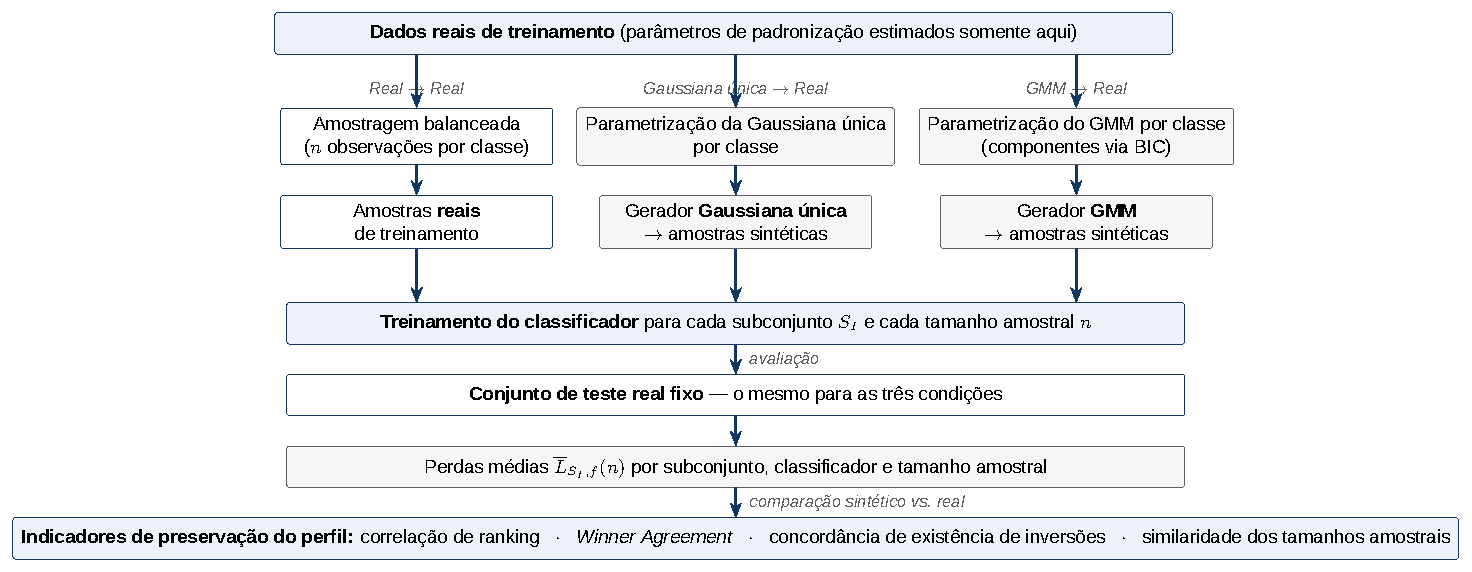
\includegraphics[width=\textwidth]{figures/conceptual/pipeline_condicoes.pdf}
  \sourcebelow{elaboração própria}
\end{figure}

\subsection{Gaussiana única por classe}

Para cada classe $c$, a Gaussiana única é parametrizada como
\begin{equation}
  Z\mid Y=c\sim\mathcal{N}(\widehat{\bm\mu}_c,\widehat{\bm\Sigma}_c),
  \label{eq:single-gaussian}
\end{equation}
em que $\widehat{\bm\mu}_c$ e $\widehat{\bm\Sigma}_c$ são, respectivamente, a média e a covariância amostrais calculadas no espaço completo dos canais, utilizando apenas os dados reais de treinamento. As covariâncias podem diferir entre classes. Quando necessário para garantir definição positiva, é adicionada uma pequena regularização diagonal, registrada nos metadados.

\subsection{Mistura gaussiana por classe}

O segundo gerador sintético é parametrizado como uma mistura finita por classe,
\begin{equation}
  p(z\mid Y=c)=\sum_{k=1}^{K_c}\pi_{ck}\,
  \mathcal{N}(z\mid\bm\mu_{ck},\bm\Sigma_{ck}),
  \label{eq:method-gmm}
\end{equation}
com pesos não negativos e soma unitária. A parametrização utiliza covariâncias completas, regularização numérica, cinco inicializações e semente fixa. São considerados de um a cinco componentes, respeitando o mínimo de 50 observações por componente; o número $K_c$ é escolhido separadamente em cada classe pelo menor BIC \cite{mclachlan2000,schwarz1978}.

A comparação entre os geradores não é formulada como um campeonato no qual o GMM deveria necessariamente vencer. Uma única Gaussiana é computacionalmente mais simples e mais interpretável. O ganho do modelo mais flexível só é relevante quando o treinamento com as amostras que ele produz modifica de modo substantivo a preservação do perfil de cooperação preditiva.

\section{Enumeração dos subconjuntos e classificadores}

Todos os subconjuntos não vazios são enumerados. Para Occupancy e Air Quality, $d=5$ e $|\mathcal{S}|=31$; para SUPPORT2, $d=7$ e $|\mathcal{S}|=127$. Diferentemente do \SLACGS, que acompanhava uma sequência incremental prefixada de dimensões, o \CoInfoSim{} compara combinações arbitrárias e pode detectar redundância ou complementaridade que não apareceria em uma única ordem de adição.

Os classificadores implementados são:

\begin{itemize}
  \item \textbf{Linear SVM}, baseline linear baseado em margem \cite{cortes1995};
  \item \textbf{Regressão Logística}, baseline probabilístico linear \cite{hosmer2013};
  \item \textbf{Gaussian Naive Bayes}, modelo probabilístico com independência condicional entre canais \cite{handyu2001};
  \item \textbf{Random Forest}, ensemble não linear de árvores \cite{breiman2001}.
\end{itemize}

Os três primeiros constituem o conjunto histórico dos cenários Occupancy e Air Quality. O Random Forest foi adicionado em uma execução específica do SUPPORT2. Como seu custo foi aproximadamente três a cinco vezes maior que o dos classificadores lineares no experimento completo, não foi executado nos outros datasets dentro do prazo. Portanto, qualquer conclusão sobre ele permanece restrita à interação entre SUPPORT2, os geradores e a configuração calibrada.

\section{Amostragem balanceada e grade de tamanhos}

Em cada replicação, o treinamento contém exatamente $n$ observações de cada classe. Essa escolha controla a quantidade de evidência disponível por classe e evita que mudanças na prevalência de treinamento sejam confundidas com o efeito de $n$. Ela não afirma que o balanceamento seja universalmente superior nem altera a prevalência do teste real, que permanece própria de cada cenário. A literatura sobre dados desbalanceados mostra que amostragem, ponderação e métricas devem ser escolhidas segundo objetivo, distribuição e custo dos erros \cite{He2009}.

A grade principal usa potências de dois. Os modos atuais estão resumidos na Tabela \ref{tab:mc-modes}. O modo \textit{full-scale} mantém a precisão do modo \textit{full}, mas estende ou limita a grade até a maior potência de dois que não excede a quantidade disponível na classe minoritária do treinamento.

\begin{table}[H]
  \centering
  \caption{Configurações dos modos de execução Monte Carlo}
  \label{tab:mc-modes}
  \begin{tabularx}{\textwidth}{l>{\raggedright\arraybackslash}Xrrrr}
    \toprule
    Modo & Grade padrão de $n$ & $R_{\min}$ & $R_{\max}$ & Lote & Alvo da meia largura \\
    \midrule
    smoke & 2, 4, 8, 16, 32 & 10 & 40 & 5 & 0,05 \\
    fast & 2 até 128 & 30 & 300 & 10 & 0,03 \\
    full & 2 até 512 & 100 & 2.000 & 20 & 0,01 \\
    full-scale & potências de 2 até a capacidade & 100 & 2.000 & 20 & 0,01 \\
    strict & 2 até 512 & 100 & 2.000 & 20 & 0,005 \\
    \bottomrule
  \end{tabularx}
  \sourcebelow{elaboração própria a partir da configuração versionada do \CoInfoSim}
\end{table}

\section{Amostras incrementalmente aninhadas}

Para cada classe $c$ e replicação $r$, é gerada uma ordem determinística de observações. O conjunto usado em um tamanho menor é prefixo do conjunto usado em qualquer tamanho maior:
\begin{equation}
  D^{(r,c)}_{2}\subset D^{(r,c)}_{4}\subset D^{(r,c)}_{8}\subset\cdots.
  \label{eq:nested-samples}
\end{equation}
No braço real, uma permutação sem reposição é fixada por classe e replicação, e cada $n$ utiliza os primeiros índices. Na Gaussiana única, o mesmo gerador pseudoaleatório e a mesma semente produzem prefixos idênticos. No GMM, cada linha consome uma escolha de componente e um bloco fixo de normais, preservando a mesma propriedade.

Esse pareamento não remove a incerteza Monte Carlo, mas reduz a variação irrelevante entre pontos consecutivos: ao passar de $n$ para $2n$, as observações anteriores são mantidas e novas observações são adicionadas. A estratégia é relacionada ao princípio de números aleatórios comuns, empregado para melhorar comparações entre configurações ao compartilhar parte da realização aleatória \cite{Kahn1953}. Aqui, o objetivo principal é isolar melhor o efeito do crescimento amostral e produzir curvas cuja oscilação não resulte da substituição integral do conjunto de treinamento.

\section{Critério adaptativo de parada}

As replicações são executadas em lotes. Após cada lote e somente quando o mínimo de replicações foi alcançado, calcula-se o erro-padrão da perda em toda célula $(S_I,f)$. Para nível normal aproximado de 95\%, a meia largura observada é
\begin{equation}
  h_{S_I,f}(n)=1{,}96\,\widehat{\mathrm{SE}}\!\left[
  \widehat{L}_{S_I,f,r}(n)\right].
\end{equation}
Define-se a pior incerteza naquele $n$ como
\begin{equation}
  h_{\max}(n)=\max_{S_I\in\mathcal{S},\,f\in\mathcal{F}}h_{S_I,f}(n).
\end{equation}
A execução para $n$ termina por convergência quando
\begin{equation}
  h_{\max}(n)\leq\varepsilon,
  \label{eq:stopping}
\end{equation}
ou por orçamento quando $R_{\max}$ é alcançado. Todas as células possuem o mesmo número de replicações no momento da decisão. O procedimento pertence à família de métodos sequenciais orientados por precisão, embora a implementação use uma regra prática em fronteiras de lote e não seja apresentada como aplicação exata de um intervalo sequencial clássico \cite{ChowRobbins1965}.

O critério evita tanto interromper regiões de alta variabilidade prematuramente quanto executar o orçamento máximo quando todas as curvas já atingiram a precisão estabelecida. Para cada $n$, o motivo da parada, o total de replicações e $h_{\max}(n)$ são persistidos.

\section{Paralelização e equivalência científica}

A carga aproximada de treinamentos de classificadores cresce com
\begin{equation}
  |\mathcal{N}|\times R\times(2^d-1)\times|\mathcal{F}|\times|\mathcal{G}|.
  \label{eq:computational-load}
\end{equation}
No SUPPORT2, cada replicação pode envolver 127 subconjuntos em cada classificador e braço. A paralelização é, portanto, uma condição prática para execuções completas.

O mecanismo de execução por processos distribui \emph{replicações completas}, e não células isoladas. Um conjunto persistente de processos de trabalho recebe o amostrador, todos os subconjuntos, o teste fixo e o plano de classificadores. Cada processo limita as bibliotecas numéricas a uma quantidade configurável de linhas de execução internas; no experimento com Random Forest, o estimador utiliza \texttt{n\_jobs=1}, evitando paralelismo aninhado e competição descontrolada por núcleos.

A quantidade efetiva de processos de trabalho é o mínimo entre o valor solicitado e o tamanho do lote. Os resultados podem terminar fora de ordem, mas são ordenados pelo identificador da replicação antes de serem incorporados ao acumulador. A regra de parada é avaliada apenas depois que o lote inteiro foi concluído. Desse modo, a execução paralela conserva as mesmas fronteiras de lote, sementes, contagens e resultados científicos da execução sequencial; o mecanismo altera o tempo de execução, não o protocolo estatístico.

\section{Calibração do Random Forest}

O Random Forest do SUPPORT2 foi calibrado uma única vez usando exclusivamente os dados reais de treinamento. A configuração aprovada é armazenada em um artefato versionado e validada por hash do arquivo bruto, impressão digital da partição, definição do alvo, ordem dos canais, semente do particionamento, versão do \textit{scikit-learn} e parâmetros do estimador.

Depois de congelada, a mesma configuração é reutilizada sem alteração nos três braços, em todos os subconjuntos, tamanhos amostrais e replicações. A política de semente do estimador depende da semente-base, do namespace do classificador e do ID da replicação; a mesma replicação utiliza, portanto, a mesma semente de Random Forest entre braços, subconjuntos e valores de $n$. Esse pareamento controla uma fonte de variabilidade interna, mas não torna iguais os dados de treinamento.

A calibração não é executada automaticamente durante um cenário, e não há configuração alternativa silenciosa quando o artefato está ausente ou incompatível. Essa separação impede que o teste real ou cada braço sintético conduza a uma configuração diferente, o que inviabilizaria a comparação do perfil de cooperação preditiva entre braços.

\section{Persistência, rastreabilidade e reprodutibilidade}

Cada execução persiste configurações científicas e computacionais, incluindo:

\begin{itemize}
  \item sementes, grade efetiva de $n$, classificadores e subconjuntos;
  \item parâmetros de padronização e definição do alvo;
  \item hashes dos arquivos brutos e impressões digitais das partições;
  \item parâmetros da Gaussiana e componentes selecionados do GMM;
  \item mecanismo de execução, processos de trabalho, linhas de execução internas e método de criação de processos;
  \item replicações, motivo de parada e meia largura máxima por $n$;
  \item versão do software, identificadores de execução e metadados de calibração.
\end{itemize}

Os diretórios de execução são identificados e tratados como imutáveis. Relatórios HTML e figuras podem ser regenerados a partir dos resultados persistidos sem repetir o Monte Carlo. A publicação online complementa o PDF: o relatório acadêmico seleciona os resultados necessários à argumentação, enquanto os artefatos completos preservam rankings por $n$, matrizes, curvas e dados de auditoria \cite{azevedo2026coinfosim}.
